% !TeX spellcheck = en_GB
\chapter{Methodological Approach} \label{chap:method-approach}

In this chapter, we will formally state the problem this work aims to address, as well as its the proposed solution. In section \ref{sec:problem} the problem statement is exposed, section \ref{sec:requirements} lists the solutions main functional, non-functional and structural requirements, section \ref{sec:arch} addresses the architecture of the solution, section \ref{sec:method} exposes the established methodology and section \ref{sec:work-plan} contains the proposed work plan.

\section{Problem Statement} \label{sec:problem}

\begin{displayquote}
	 \textit{The reviewed literature addressing solutions to sequential decision-making problems in graph-based environments is sparse and scarce, leading to a research gap for comparative and systematic \ac{GRL} approaches analysing scalability under different sized scenarios and adaptability to topology variation.}
\end{displayquote}

As addressed in the previous chapter, graphs are ubiquitous representations that can serve to instinctively represent several problems and their objects. In some network-oriented domains, these representations reveal underlying features that can't be naturally represented by plain Euclidean data. This problem becomes even more difficult considering that graph data is complex and sparse, something that brings the need for methods that efficiently extract representations. \par
By conducting a thorough literature review of the relevant studies in this context, we observed that current \ac{RL} algorithms are not as efficient as \ac{GRL} techniques in handling such complex environments, because of not considering and generalizing environment topology features in the decision-making process. This deeply affects the performance of decision systems inserted in network-oriented domains where the intricate relationships between the objects may be relevant for mapping the observable environment states to optimal action policies. \par
More and more \ac{GRL} attracts the curiosity of academics, only increasing the relevance of this problem. With the recent advancements of \acp{GNN}, the popularity around \ac{GRL} has risen because of their excellent efficiency in creating optimal graph representations and other graph machine learning problems. However, with \ac{GRL} being a field whose research is still in initial phase, the gathered literature is very sparse, with a lack of works addressing the benefits, disadvantages and performance of the various proposed models. Moreover, the literature also highlights the importance of studying \ac{GRL} models in scenarios under topology variations and of different sizes for analysing their scalability. \par

\subsection{Scope}

This dissertation will focus on studying this problem in the context of single-agent \ac{RL} algorithms, given that multi-agent systems are significantly more complex to implement. Furthermore, in the context of the dissertation's application domain, which is smart grid services, the possible improvements in \ac{GRL} techniques will be implemented to the \acf{DED} problem that studies solutions that optimize power generation cost while maintaining reliable grid stability. Additionally, the \ac{GRL} proposed models may be also implemented to solve other smart grid systems such as Undervoltage Load Shedding and Volt-VAR Regulation.

\section{Problem Formalization}

In this section, the main problem of study of this dissertation is formally introduced. Firstly, the problem is approached from an application domain perspective, uncovering the details of the \ac{DED} problem and its main features. In the sequent subsection, the \ac{DED} problem is formalized as a dynamic sequential decision-making problem, and its characteristics are presented under the form of its corresponding \ac{MDP}.

\subsection{Dynamic Economic Dispatch}

\begin{comment}
	* Citation Needed (?)
	* Revise
	* Constraints
	
	
	
	
	
	
	
\end{comment}

\begin{center}
	\begin{tabular}{ | m{2cm} | m{10cm}| } 
		\hline
		$F(t)$ & Total Operational Cost \\ 
		\hline
		$F_\text{NRES}(t)$ & Total Non-Renewable Generators Operational Cost \\
		\hline
		$F_\text{NRES}(t)$ & Total Renewable Generators Operational Cost \\
		\hline
		$F_\text{ESS}(t)$ & Total ESS Operational Cost \\
		\hline
		$T$ & Terminal Timestep \\
		\hline
		$t$ & Timestep \\
		\hline
		$c^\text{NRES}_i$ & Cost of conventinal generator $i$ in €/MWh \\
		\hline
		$P^\text{NRES}_i(t)$ & Current generated power of non-renewable generator $i$ in MW \\
		\hline
		$\beta_\text{RES}$ & \ac{RES} wasted energy penalty term \\
		\hline
		$P^\text{RES}_i(t)$ & Current generated power of renewable generator $i$ in MW \\
		\hline
		$\overline{P^\text{RES}_i}(t)$ &  Current power of renewable generator $i$ before curtailmentin MW \\
		\hline
		$c^\text{ESS}_i$ & Operational Cost of \ac{ESS} $i$ in €/MW \\
		\hline
		$P^\text{ESS}_i(t)$ & Discharging/Charging Power of \ac{ESS} $i$ \\
		\hline
		$P^\text{LOAD}_i(t)$ & Active Power demand of load $i$ \\
		\hline
		$Q^\text{LOAD}_i(t)$ & Reactive Power demand of load $i$ \\
		\hline
		$F_i$ or $F_{i,j}$ & Powerline $i$ status \\
		\hline
		$\text{rho}_i$ or $\text{rho}_{i,j}$ & Relative flows of powerline $i$ or with origin in substation $i$ and destination in substation $j$. Ratio of the flow divided by its thermal limit. \\
		\hline
		$P^\text{G}_i(t)$ & Current generated active power of generator $i$ in MW \\
		\hline
		$Q^\text{G}_i(t)$ & Current generated reactive power of generator $i$ in MW \\
		\hline
		$N$ & Number of non-renewable generators \\
		\hline
		$M$ & Number of renewable generators \\
		\hline
		$K$ & Number of loads \\
		\hline
		$L$ & Number of powerlines \\
		\hline
	\end{tabular}
\end{center}

\subsubsection{Objective Function}

The \ac{DED} problem addresses the issue of balancing the necessity for ensuring stability, security and reliability of a power grid while also minimizing its operating cost. This problem is hardened by the paradigm observed in current power systems where \ac{ESS} and \ac{RES} are available and also need to be taken in consideration when studying solutions for this problem. \par
In the idealized power system, the main components taken into account are renewable and non-renewable generators, loads, powerlines, substations and storage systems.
Equation \ref{eq:ded-function} highlights the main objective function for the \ac{DED} problem and is composed of three main components: $F_\text{NRES}(t)$ represents the cost of energy produced by conventional generators, $F_\text{RES}(t)$ is the term that depicts the cost of wasted energy from \ac{RES} and $F_{\text{ESS}}(t)$ the \ac{ESS} operation cost. \par

\begin{equation} \label{eq:ded-function}
 \min\sum^T_{t=1}(F_\text{NRES}(t) + F_{\text{RES}}(t) + F_{\text{ESS}}(t))
\end{equation}

Conventional generation cost calculation is presented in equation \ref{eq:conv-cost}. For the sake of simplicity, this component is reduced to a linear equation and represented by a static $c_i$ term for generator $i$ in €/MWh . Regarding the cost of wasted \ac{RES} energy, a penalty term $\beta_\text{RES}$ is introduced that defines a cost for the abandoned renewable energy. Lastly, concerning \acp{ESS}, the cost is directly related to its operation cost $c^\text{ESS}_i$ in €/MW and to its current discharging/charging power $P^\text{ESS}_i$ with a positive power meaning that energy is being absorbed.

\begin{equation} \label{eq:conv-cost}
	F_\text{NRES}(t) = \sum^N_{i=0} c^\text{NRES}_i P^\text{NRES}_i(t) \Delta t
\end{equation}

\begin{equation} \label{eq:res-cost}
	F_\text{RES}(t) = \beta_\text{RES} \sum^M_{i=0}  (\overline{P^\text{RES}_i}(t) - P^\text{RES}_i(t)) \Delta t 
\end{equation}

\begin{equation} \label{eq:ess-cost}
	F_\text{ESS}(t) = \sum^O_{i=0} c^\text{ESS}_i P^\text{ESS}_i(t) 
\end{equation}



\subsubsection{Constraints}

In order to maintain stability and reliable power distribution, the system must follow several operational constraints. These restrictions are related to generators, voltage, powerlines and its overall stability.  \par

The main rule in a power system environment consists in the compliance with power balance. This  implies that, at all times, the sum of production output of all generators must surpass the total system load demand, as portrayed by equation \ref{eq:c-power-balance}. 

\begin{equation} \label{eq:c-power-balance}
	\sum^N_i P^\text{NRES}_i(t) + \sum^M_i P^\text{RES}_i(t) = \sum^L_i P^\text{LOAD}_i(t) + \delta, \delta > 0
\end{equation}

Considering non-renewable generations, its output value it is bounded by absolute maximum and minimum values respective to each generator, $\underline{P^\text{NRES}_i}$ and $\overline{P^\text{NRES}_i}$, as depicted in equation \ref{eq:prod-limits}. Furthermore, as illustrated in equation \ref{eq:ramp-limits}, the varying power between two different timesteps is also restricted by maximum ramp up and down limits, $\underline{\eta_i }$ and $\overline{\eta_i }$. \par

\begin{equation} \label{eq:prod-limits}
	\forall t, i: \underline{P^\text{NRES}_i} \leq P^\text{NRES}_i(t) \leq \overline{P^\text{NRES}_i}
\end{equation}

\begin{equation} \label{eq:ramp-limits}
	\forall t, i: \underline{\eta_i } \Delta t \leq P^\text{NRES}_i (t + 1) - P^\text{NRES}_i (t) \leq \overline{\eta_i} \Delta t
\end{equation}

In contrast with these static production limits, renewable generator production limits are dynamic. Depending on the type of \ac{RES}, the maximum available generation output is subject to the environmental characteristics dictated by the environment. In such manner, the ouput value of renewable generations for any timestep $t$ is bounded by a maximum production value, $\overline{P^\text{RES}_i} (t)$ and 0. Equation \ref{eq:res-limits}

\begin{equation} \label{eq:res-limits}
	\forall t, i: 0 \leq P^\text{RES}_i (t) \leq \overline{P^\text{RES}_i} (t)
\end{equation}

Regarding powerlines, there are two thresholds that restrict their operation in cases of line overflow. They are applied to safeguard the condition of powerlines and emulate the behaviour of a real power system $\text{rho}$, in two difference scenarios:
\begin{itemize}
	\item \textbf{Hard Overflow} - In case the relative flow of any powerline surpasses the hard overflow threshold, $\theta_\text{hard},$ it's instantly disconnected. This is known as time overcurrent;
	\item \textbf{Soft Overflow} - A line is allowed to surpass the soft overflow threshold, $\theta_\text{soft}$, for $T_\text{soft}$ timesteps before being disconnected for safety reasons. This consists in an instantenous overcurrent;
\end{itemize}
In any case, when a powerline is disconnected for safety reasons, it's affected by a reconnection cooldown, $T_\text{reconnect}$.

\begin{comment}
	Flow constraints ?
	Voltage Constraints ? 
\end{comment}

\subsection{\acf{MDP}}

In this section, the \ac{DED} problem is formalized in the as a sequential decision-making problem and its \ac{MDP} is uncovered. 

\subsubsection{Simple}

\begin{description}
	\item[Action] The considered action space includes the change in conventional generator redispatching $\Delta P^G_i$, renewable energy curtailment $P^\text{RES}_i$ and \ac{ESS} absorption/production power $P^\text{ESS}_i$.
	
	\item[Observation] The observation space is composed of four components regarding Generators, \ac{RES}, Loads and Powerlines, highlighted in the following equations:
	
	\begin{comment}
		* Voltage
	\end{comment}
	
	\begin{equation} \label{eq:simple-obs-space1}
		o_{1}(t)= \begin{bmatrix}
			P^\text{NRES}_1 & P^\text{NRES}_2 & \dots & P^\text{NRES}_{N} \\
		\end{bmatrix}
	\end{equation}
	
	\begin{equation} \label{eq:simple-obs-space2}
		o_{2}(t)= \begin{bmatrix}
			P^\text{RES}_1 & P^\text{RES}_2 & \dots & P^\text{RES}_{M} \\
			\overline{P^\text{RES}_1} & \overline{P^\text{RES}_2} & \dots & \overline{P^\text{RES}_{M}} \\
		\end{bmatrix}
	\end{equation}
	
	\begin{equation} \label{eq:simple-obs-space3}
		o_{3}(t)= \begin{bmatrix}
			P^\text{LOAD}_1 & P^\text{LOAD}_2 & \dots & P^\text{LOAD}_{K} \\
			Q^\text{LOAD}_1 & Q^\text{LOAD}_2 & \dots & Q^\text{LOAD}_{K} \\
		\end{bmatrix}
	\end{equation}
	
	\begin{equation} \label{eq:simple-obs-space4}
		o_{4}(t)= \begin{bmatrix}
			F_1 & F_2 & \dots & F_{L} \\
			\text{rho}_1 & \text{rho}_2 & \dots & \text{rho}_{L} \\
		\end{bmatrix}
	\end{equation}
	
	\begin{equation} \label{eq:simple-obs-space}
		o(t)= \{ o_{1}(t), o_{2}(t), o_{3}(t), o_{4}(t) \}
	\end{equation}
	
	This tuple encompasses the main elements of the powergrid an their characteristics, without capturing their topology.
	
	\item[Reward] 
	
	\begin{equation}
		r(t) = r_1(t) + r_2(t)
	\end{equation}
	
	\begin{equation}
		\begin{split}
			r_1(t) &= \overline{F_\text{NRES}} - F_\text{NRES}(t) \\
			&= \overline{F_\text{NRES}} - \sum^N_{i=0} c^\text{NRES}_i P^\text{NRES}_i(t) \Delta t
		\end{split}
	\end{equation}
	
	\begin{equation}
		\begin{split}
			r_2(t) &= - F_\text{RES}(t) \\
			&= \beta_\text{RES} \sum^M_{i=0} (\overline{P^\text{RES}_i}(t) - P^\text{RES}_i(t)) \Delta t
		\end{split}
	\end{equation}
\end{description}


\subsubsection{Graph}

\begin{description}
	\item[Action] The considered action space includes the change in conventional generator redispatching $\Delta P^G_i$, renewable energy curtailment $P^\text{RES}_i$ and \ac{ESS} absorption/production power $P^\text{ESS}_i$.
	
	\item[Observation] The observation space includes the current active and reactive load power, conventional and \ac{RES} generator active power, \ac{RES} power before curtailment, state-of-charge of \ac{ESS} and the current timestep for each node of the grid, respectively represented as a tuple in equation \ref{eq:graph-obs-space}.
	
	\begin{equation} \label{eq:graph-obs-space}
		o_i(t) = \{P^\text{LOAD}_i, Q^\text{LOAD}_i, P^\text{NRES}_i, P^\text{RES}_i, \overline{P^\text{RES}_i}, t\}
	\end{equation}
	
	Beyond that, the observation also includes the topology of the power grid as a graph structure, considering the current powerline status as edges connecting substations and their respective relative flow as their weights. In this manner, the full observation is represented as:
	
	\begin{equation}
		o(t) = G(\text{Adj}, W, X)
	\end{equation}
	
	where 
	
	\begin{equation}
		\text{Adj}_{i,j} = F_{i,j}
	\end{equation}
	
	\begin{equation}
		W_{i,j} = \text{rho}_{i,j}
	\end{equation}
	
	\begin{equation}
		X_i = o_i
	\end{equation}
	
	\item[Reward] description
	
	\begin{equation}
		r(t) = r_1(t) + r_2(t)
	\end{equation}
	
	\begin{equation}
		\begin{split}
			r_1(t) &= \overline{F_\text{NRES}} - F_\text{NRES}(t) \\
			&= \overline{F_\text{NRES}} - \sum^N_{i=0} c^\text{NRES}_i P^\text{NRES}_i(t) \Delta t
		\end{split}
	\end{equation}
	
	\begin{equation}
		\begin{split}
			r_2(t) &= - F_\text{RES}(t) \\
			&= \beta_\text{RES} \sum^M_{i=0} (\overline{P^\text{RES}_i}(t) - P^\text{RES}_i(t)) \Delta t
		\end{split}
	\end{equation}
	
\end{description}

\begin{comment}
	* TODO
\end{comment}


\section{Architecture} \label{sec:arch}

Considering the conclusions taken from the reviewed literature, in chapter \ref{chap:literature-review}, our proposed solution combines efficient \acf{DRL} approaches with \acfp{GNN}, the state-of-the-art approach for graph representation learning. Generally, the system receives graph-based representations of the environment and encodes them using the \ac{GNN} algorithm. By also leveraging deep learning techniques, \ac{DRL} maps the encoded embeddings to optimal action sequences with the goal of meeting the real-time load demand and reducing the operating cost of the power distribution grid. The general architecture of the solution can be observed in figure \ref{fig:arch}.

\begin{figure}
	\centering
	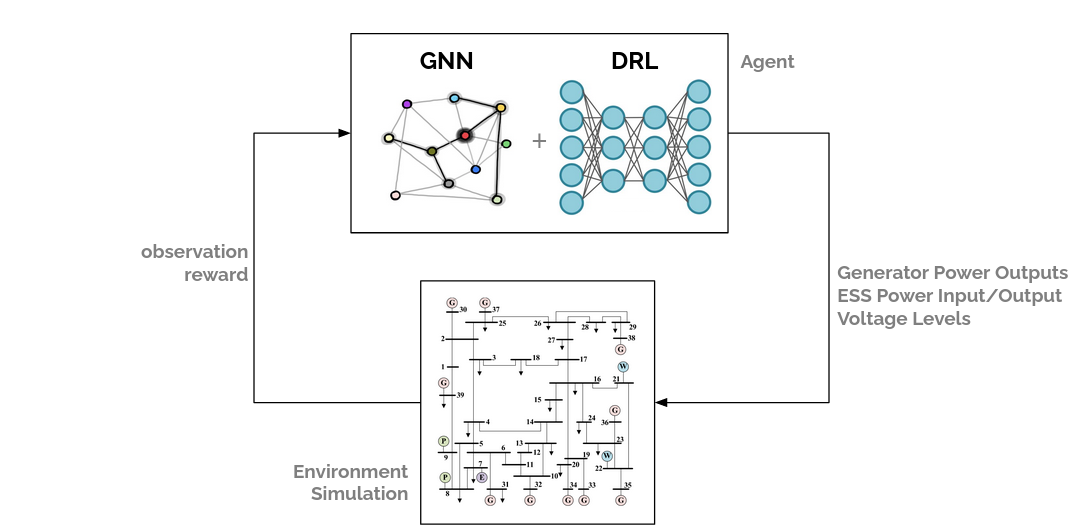
\includegraphics[width=0.85\linewidth]{./figures/arch.png}
	\caption{Solution Architecture}
	\label{fig:arch}
\end{figure}


To fulfil this, the agent adjusts the generator power output and voltage levels and manages the \ac{ESS} operation in real-time. \par
The solution is executed in the context of a power grid simulation that models the appropriate elements, properties, constraints and operating of the power distribution grid. This method is further described in the upcoming subsection \ref{sec:method}.



\section{Evaluation Metrics} \label{sec:eval-methods}

\begin{comment}
	* Sample Efficiency
	* Other methods
	* Equations
	* TODO
\end{comment}


The solution described in the previous subsections \ref{sec:arch} and \ref{sec:method} clearly involves intricate operational mechanisms, something that calls for a sophisticated evaluative process. Furthermore, given the comparative nature of this dissertation the evaluation and analysis methods will be key factors in studying and confronting the different combinations of \acp{GNN} and \ac{DRL}, as well as possible improvements in the integration of these techniques.
In this manner, we define the four dimensions for evaluating and analysing the different \ac{GRL} models:

\begin{description}
	\item[Learning efficiency] This dimension assesses how effectively the models learn and improve their decision-making process over time. It involves evaluating how quickly they converge to optimal or near-optimal dispatch strategies through the convergence rate. 
	
	\item[Computational Efficiency] It's crucial that the solution is able to perform well on real-time execution. In this context, not only it's important to assess the solution's decision computation performance but also to measure the time necessary for the model offline training, as well as the observed CPU/GPU resource utilization.
	
	\item[Dispatch Efficiency] The performance of the \ac{GRL} model in managing power distribution from the various generators will be mainly measured by the average operating cost (in \textit{Euros}) derived from the agent's sequence. Furthermore, other system behaviours will be analysed such as Renewable Energy Source Penetration, through the average ratio of maximum power and real power output, and \ac{ESS} utilization, through the average energy stored.
	
	\item[Scalability and Adaptation]  The solution will be applied to scenarios of several sizes for analysing its scalability. Furthermore, we will induce variations in the simulation scenarios to test the model's ability to handle topology changes.
\end{description}


\begin{comment}
	* TODO
\end{comment}

\section{Technologies}

Beyond being a well-documented, fast, robust and modular language, \textit{Python} is an ubiquitous technology for implementing machine learning algorithms. Furthermore, the main libraries used to implement the simulation environment and algorithm are native to this language.
\par
In table x, the main requirements for the project can be observed, along with their respective version number and a short description of their purpose and functionality.
\par

\begin{table}
	\begin{tabular}{|l|l|l|}
		\hline
		\textbf{Name} & \textbf{Description} & \textbf{Version Number} \\
		\hline
		Python & Functional Programming Language & 3.11.9 \\
		\hline
		Numpy & Numerical Computing Library& 1.24.3 \\
		\hline
		Ray & Used for hyperparameter tuning & 2.21.0 \\
		\hline
		PyTorch & \acs{ML} Library used by stable-baselines3 & 2.3.0 \\
		\hline
		PyTorch Geometric & \ac{GNN} Implementations & 2.5.3 \\
		\hline
		Grid2Op & Power Grid Simulation Platform & 1.9.8 \\
		\hline
		Pandas & Data Manipulation and Analysis & 1.5.3 \\
		\hline
		LightSim2Grid & Fast Grid2Op Backend & 0.8.2 \\
		\hline
		Gymnasium & \ac{RL} Single-Agent API & 0.29.1 \\
		\hline
		Stable Baselines 3 & \ac{DRL} Implementations & 2.3.2 \\
		\hline
	\end{tabular}
	\caption{Project Requirements}
\end{table}

Grid2Op is a critical requirement used to simulate the power grid operation in different manageable scenarios. This is further discussed in the next subsection \ref{sec:simulation-env}. Stable-Baselines3 was chosen for its performance, customization and descriptive documentation, while PyTorch Geometric was favoured because of the wide variety of \acp{GNN} Implementations included. Additionally, these libraries mix well because stable-baselines3 already uses PyTorch in its \ac{DRL} implementations.
\par
Lastly, \textit{Gymnasium} is used as the standard \ac{RL} single-agent API in the entirety of the project, adding robustness, scalability and flexibility to agent-environment interaction process in the implementation.  \par

\section{Simulation Environment} \label{sec:simulation-env}

The \textit{Grid2Op} framework \cite{rtefranceGrid2OpDocumentation} will be used for modelling the sequential decision-making process on simulated power distribution grids. \textit{Grid2Op} is designed by RTE (\textit{Réseau de Transport d'Électricité}), the electricity transmission system operator of France, and is equipped with a variety of pre-defined scenarios used in coding competitions and based on real-world data \cite{rtefranceGrid2OpDocumentation}. \par
This \textit{python} library implements the creation of power grid environments that emulate a subset of the elements and physical constraints of real power systems. On one hand, the main objects and their interactions are captured realistically, while on the other, the abstraction level used to model the fundamental elements of a power grid facilitates the implementation of intelligent systems in safe and controllable scenarios. \par
Furthermore, \textit{Grid2Op} models the dynamic topology of power systems as graph-structured data, which also eases the study of how this information can influence decision-making systems performing on these environments.  In figure \ref{fig:grid2op-graph}, a graphical plot of the environment state at an arbitrary timestep can be observed. \par
This framework is compatible with the \textit{Gymnasium} framework \cite{faramafoundationGymnasiumDocumentation}, a widely used toolkit for developing \ac{RL} algorithms, which will also will be used in this work together with the Grid2Op simulation environment. 

\begin{itemize}
	\item redispatch - change the production output of non-renewable generators in incrementing or decrementing intervals 
	\item curtail - change the production setpoint of renewable generators bellow the current maximum available power \cite{rtefranceGrid2OpDocumentation}
\end{itemize}



\begin{figure}
	\centering
	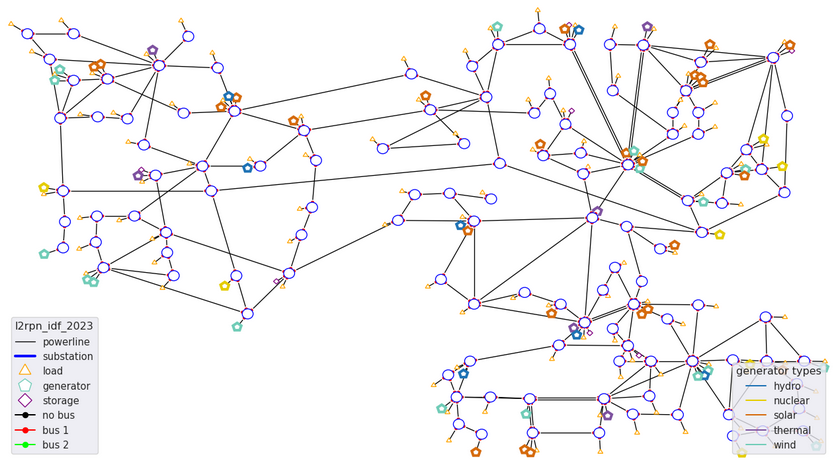
\includegraphics[width=0.85\linewidth]{./figures/grid2op-graph.png}
	\caption{Grid2Op \textit{l2rpn\_idf\_2023} 118-bus test case \cite{rtefranceGrid2OpDocumentation}}
	\label{fig:grid2op-graph}
\end{figure}


\subsection{Elements}

The main elements that are modelled by the simulation environment are presented in this subsection. The power grid is reduced to its fundamental components and their properties:

\begin{itemize}
	\item \textbf{Buses} are the fundamental objects of the power grid, representing nodes where power sources, loads and other elements are connected\cite{rtefranceGrid2OpDocumentation}.
	
	\item \textbf{Powerlines} represent edges in the power grid and connect the different buses together. They represent the physical transmission and distribution lines and allow power to flow from one part of the grid to another \cite{rtefranceGrid2OpDocumentation}.
	\begin{itemize}
		\item status
		\item rho
	\end{itemize}
	
	\item \textbf{Generators} are critical grid elements connected to buses whose main role is to produce power and maintain grid stability by balancing the energy supply and demand. They can be Conventional Thermal Generators, Wind Turbines or Photovoltaic Cells \cite{rtefranceGrid2OpDocumentation}.
	\begin{itemize}
		\item $P^\text{NRES}_i(t)$ - Power generation at non-renewable generator $i$
		\item $P^\text{RES}_i(t)$ - Power generation at renewable generator $i$
		\item $\overline{P^\text{RES}_i}(t)$ - Maximum power generation at renewable generator $i$
		\item $\overline{P^\text{NRES}_i}, \underline{P^\text{NRES}_i}$ - Maximum/Minimum power generation at renewable generator $i$
	\end{itemize}
	
	
	\item \textbf{Loads} consume power from the grid, simulating electricity use. They're also associated to an individual bus \cite{rtefranceGrid2OpDocumentation}.
	\begin{itemize}
		\item $P^\text{LOAD}_i$ - Active power at load $i$
		\item $Q^\text{LOAD}_i$ - Reactive power at load $i$
	\end{itemize}
	
	\item \textbf{Storage Units} can act as both consumers and producers. They're able to retain energy from the power grid when production surpasses demand for later injecting back power when convenient. Storage units are bound by a maximum energy storage capacity \cite{rtefranceGrid2OpDocumentation}.
\end{itemize}


Beyond \textit{grid2op} to build and run the test cases and \textit{gymnasium} as the RL framework, this project will use \textit{PyTorch} \cite{pytorchPyTorch} with \textit{PyTorch Geometric} \cite{pygteamPyGPytorch_geometric} library for developing the \ac{GNN} because of its extensive list of available implemented models. The different combinations of algorithms will be applied to a set of modified scenarios that fulfil the settled requirements. For Deep Reinforcement Learning algorithms, solutions with plain \ac{SAC}, \ac{DDPG} and \ac{PPO} approaches and combined with the \ac{GCN}, \ac{GAT} and \ac{GIN} architectures.  \par
Concerning result analysis, it's also important to point out the use of quantitative methods for evaluating the different implemented models, a topic that is further explored in the following section \ref{sec:eval-methods}.

\section{Scenarios}

\begin{table}[H] 
	\centering
	\caption{Test Case Sizes}
	\begin{tabular}{|P{2cm}|P{3.5cm}|P{3.5cm}|  }
		\hline
		& \textbf{l2rpn\_icaps\_2021} & \textbf{l2rpn\_idf\_2023} \\
		\hline
		\textbf{Buses} & 36 & 118 \\
		\hline
		\textbf{Powerlines} & 59  & 186  \\
		\hline
		\textbf{Generators} & 22 & 62  \\
		\hline
		\textbf{Loads} & 37 & 99 \\
		\hline
	\end{tabular}
	\label{tab:test-case}
\end{table}

This work will use the pre-defined \textit{grid2op} \textit{l2rpn\_icaps\_2021} and \textit{l2rpn\_idf\_2023} test environments, a modified case studies based on the original IEEE 118-bus system test case \cite{christiePowerSystemsTesta} of 36 and 118 buses, respectively. The first test case is a subset of the original 118-bus system with 50 years worth of data divided into independent \footnote{non-consecutive} weekly scenarios, while in the second case the system was modified to accommodate the \textit{possible energy mix} of France in 2035, containing 16 years of data \cite{rtefranceGrid2OpDocumentation}. The scenarios document the loads and productions at each time step, the grid layout (for display purposes), generator and \ac{ESS} characteristics \cite{rtefranceGrid2OpDocumentation} for a weekly episode, the sizes of test cases can be further observed in table \ref{tab:test-case}. In addition, the test cases data will be modified to reflect the defined requirements of this work. \par
